% TeX root = ../../paper.tex

\section{Introduction}

Petri nets are not only a graphical modeling tool but also a formal method with strict grammar and semantic definitions that can be used to model and describe the system effectively at the same time. Therefore model-based testing techniques with petri net can be used to develop tests of systems based on formal criteria to find errors at early stages in development.

\begin{figure}
  \centering
  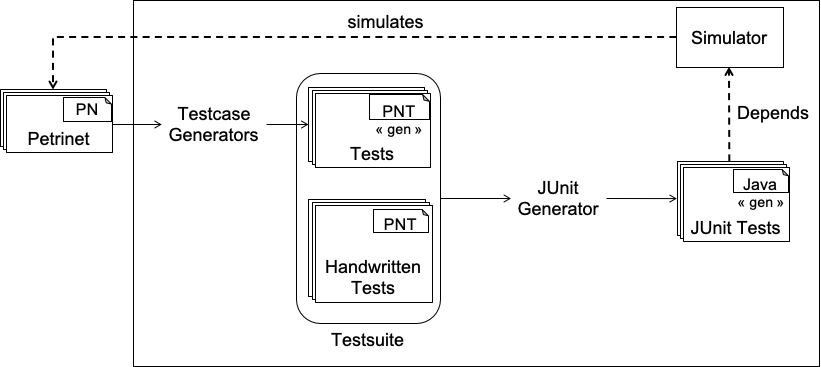
\includegraphics[scale=0.4]{src/pic/arch.png}
  \caption{The \emph{Petrinets Testing} language Architecture}
  \label{fig:arch}
\end{figure}

Based on the MontiCore Language Workbench \cite{monticore2020}, we propose the textual modeling language \emph{Petrinets Testing}. There are four main components in our \emph{Petrinets Testing} project, they are \emph{Testcase Generator}, \emph{Petrinets Testing language}, \emph{JUnit Test Generator} and \emph{Simulator}. The architecture of \emph{Petrinets Testing} project is in Fig \ref{fig:arch}. The specific responsibilities of each part are as follows:

\begin{itemize}
    \item \emph{Testcase Generator}: Any petri net model can be used as an input for the \emph{Petrinets Testing} project. First, we will use the \emph{petrinets4analysis} language to parse the given petri net model. Through the parsed petri net model, the system can automatically generate test cases using the algorithm we set, which will be mainly introduced in chapter \ref{sec:automatically generates testcase}. Furthermore, we can also create test cases manually according to the grammar of \emph{Petrinets Testing} language. Finally we will get a \emph{Petrinets Testing} model. \\
    
    \item \emph{Petrinets Testing language}: \emph{Petrinets Testing} is a domain-specific language (DSL) that is easily usable by domain experts without knowledge of programming. The grammar of the \emph{Petrinets Testing} language is defined by the MontiCore Language Workbench \cite{rumpe2017monticore}, which produces Java classes for the abstract syntax tree (AST) as well as additional infrastructure by our defined keywords and syntactic sugar in the MontiCore Language Workbench. In \emph{Petrinets Testing} language, we can define the initial markings, simulated transitions and expected markings of given petri net model. Each petri net model will have a corresponding \emph{Petrinets Testing} model (an example is in Listing \ref{lst:pnt-Cheap Cookie Machine}). Through the \emph{Petrinets Testing} language, we can define multiple test cases in the same model. \\
    
    \item \emph{JUnit Test Generator}: The petri net test needs to use JUnit, which is a simple framework to write repeatable tests, so the function of the {JUnit Test Generator} model is to convert the generated \emph{Petrinets Testing} model into a JUnit class. In each of JUnit class, we also add some auxiliary functions for the next simulation operation. \\
    
    \item \emph{Simulator}: After the program has generated \emph{Petrinets Testing} models for all petri nets, this module \emph{Simulator} will automatically execute the corresponding JUnit class for petri net testing. In the process of running, the program will first need the parsed petri net model of \emph{petrinets4analysis} language, so the \emph{petrinets4analysis} language is also used in this process. When the results of each JUnit class running meets the expected conditions, the system will finally give a "pass" signal.
\end{itemize}